\chapter{Estudio Integral de Sistemas de Riego I}

\section{Sistemas de producción Hidroagrícola}

\begin{figure}[h!]
\centering
  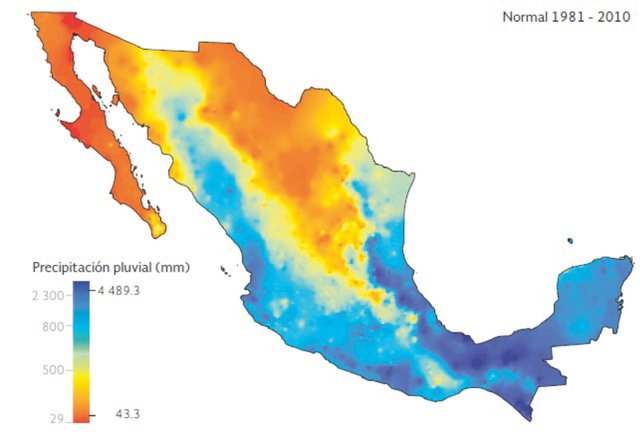
\includegraphics[width=0.5\textwidth]{ei1.jpg}
  \caption{Distribución de la precipitación pluvial, 1981-2010(mm)}
  \label{ei1}
\end{figure}
¿Por qué se requiere regar? hay dos eventos meteorológicos: la precipitación y la evaporación, a esto se le llama Oferta hídrica.
% El día cero llegó
\begin{remark}
    Si la evaporación es mayor que la precipitación, se debe regar.
\end{remark}
El agua que llega en forma natural, a través de la lluvia, se pierde por la evaporación y no queda suficiente para satisfacer las necesidades de las plantas.
% La evaporación > transpiración
\begin{definition}[Irrigación]
    Es el conjunto de técnicas y obras que permiten la aplicación controlada (cuándo y cuanto) del agua a los terrenos agrícolas, para satisfacer las necesidades de un cultivo no abastecido en forma natural.
\end{definition}
% ingeniería civil, hidrologos, geohidrologos, agrónomos, meteorologos computologos
\begin{definition}[Sistema de irrigación (Distrito de riego)]
    Es un conjunto de obras, dispositivos y artificios necesarios para captar, conducir, distribuir y aplica del agua a los suelos donde se encuentran las plantas cultivadas, proveniente de determinada fuente de abasto utilización racional y eficiente.
\end{definition}
fuente de abastecimiento (Superficial  o subterránea) se conduce a la zona de riego en un canal principal en un tramo muerto, esa es la zona de conducción; ahora de la zona de riego hay una red de distribución con canales laterales, ramales etc. luego tiene una red de drenaje para evitar las sales que por capilaridad sube del manto freático y deposita las sales; la red y sistemas de comunicaciones y de caminos.
% En México hay 87 distritos (3 millones de Ha) y es público mientras que hay 40,000 unidades de riego (3.5 millones de Ha) y es privado
\begin{definition}[Distrito de temporal tecnificado]
    Es un Área geográfica destinada normalmente a las actividades agrícolas que no cuentan con infraestructura de riego, en la cual mediante el uso de diversas técnicas y obras, se aminoraron los daños a la producción por causa de ocurrencia de lluvias fuertes prolongadas, estos también denominados distritos de drenaje o en condiciones de escasez, se aprovecha con mayor eficiencia la lluvia y la humedad en los terrenos agrícolas, el distrito de temporal tecnificado está integrado por unidades de temporal.
\end{definition}
Es un esquema típico de régimen hídrico de una zona idónea para estableces un DTT, se entiende que en dichas estas zonas hay un periodo de lluvias suficiente para producir un cultivo sin necesidad de riego más bien habría necesidad de drenar los excedentes. En la práctica la agricultura, tanto de temporal como de riego, en temporadas de lluvias se enfrenta a lis mayores ataques de plagas, enfermedades y siniestro relacionados con la precipitación.
\subsection{Distrito de Temporal Tecnificado}
México tiene un potencial agrícola de 22 millones de Ha, de las cuales 7.5 millones se ubican en las zonas del trópico húmedo y subhúmedo; su característica principal es el efecto de las altas precipitaciones que rebasan los límites de permeabilidad y retención de humedad de los suelos, lo que aunado a la falta de un sistema de drenaje natural propician inundaciones.

Con propósito de incorporar las zonas agrícolas del trópico húmedo y subhúmedo al desarrollo nacional mediante el abastecimiento de alimentos que demanda la población, desde 1947 se han hecho diversos esfuerzos por parte del gobierno federal; tales como la creación de las comisiones ejecutivas por cuencas, entre ellas, la del Papaloapan y Grijalva-Usumacinta; así como el Plan Hidráulico de la costa de Chiapas y el programa de desarrollo rural integrado del trópico húmedo (PRODERITH); las principales actividades que llevó a cabo PRODERIT (1978-1994):
\begin{enumerate}
    \item Conservación, rehabilitación de infraestructura y control de inundaciones
    \item Asesoría técnica especializada, que incluye la organización de los usuarios
    \item Transferencia a los usuarios de infraestructura, maquinaria, equipo y funciones
    \item Manejo del agua y preservación del suelo
    \item Comunicación rural, capacitación y divulgación
\end{enumerate}

Las áreas beneficiados con infraestructura de drenaje, caminos, bordos de protección y estructuras de cruce, se organizaron y se delimitaron en ámbitos territoriales, constituidos en ``Distritos de temporal tecnificado''. Estos distritos se establecen mediante acuerdo de creación con el propósito de iniciar francamente su etapa de operación y principalmente la conservación de la infraestructura y el manejo del agua y preservación del suelo. De esta manera el 7 de diciembre de 1971 se establece legalmente el primer DTT.

A partir de 1991 se inicia el proceso de transferencia de la infraestructura, maquinaria y equipo para su conservación a los usuarios, a través de un ``Contacto de prestación de servicios''

Artículo 76: El ejecutivo Federal, por conducto de la ``Comisión'', la cual se apoyará en los organismos de Cuenca, y con la  participación de los usuarios, promoverá y fomentará el establecimiento de unidades de temporal tecnificado incluyendo las de drenaje, conforme a lo asentado en el inciso b de la fracción XXV del Artículo 3 de la presente Ley, a efecto de incrementar la producción agropecuaria.

Definición de la Ley de aguas Nacionales según lo asentado en la fracción XXV, inciso b del artículo 3.

\begin{definition}[Distrito de Temporal tecnificado]
    Es un área geográfica destinada normalmente a las actividades agrícolas que no cuentan con infraestructura de riego, en la cual mediante el uso de diversas técnicas y obras, se aminoraron los daños a la producción por causa de ocurrencia de lluvias fuertes prolongadas - estos también denominados Distritos de Drenaje- o en condiciones de escasez, se aprovecha con mayor eficiencia la lluvia y la humedad en los terrenos agrícolas; el Distrito de Temporal Tecnificado está integrado por unidades de temporal
\end{definition}
La definición vigente se pude entender con base en el régimen hídrico del trópico húmedo que tiene un comportamiento de drenado.

Se entiende que en estas zonas hay un periodo de lluvias suficientes para producir un cultivo sin necesidad de riego, más bien habría necesidad de drenad los excedentes.

En la práctica la agricultura, tanto de temporal como de riego, en temporadas de lluvias se enfrenta a los mayores ataques de plagas, enfermedades y siniestros relacionados con la precipitación
% PONER MAPA DE DISTRITO DE TEMPORAL TECNIFICADO
\begin{figure}[h!]
\centering
  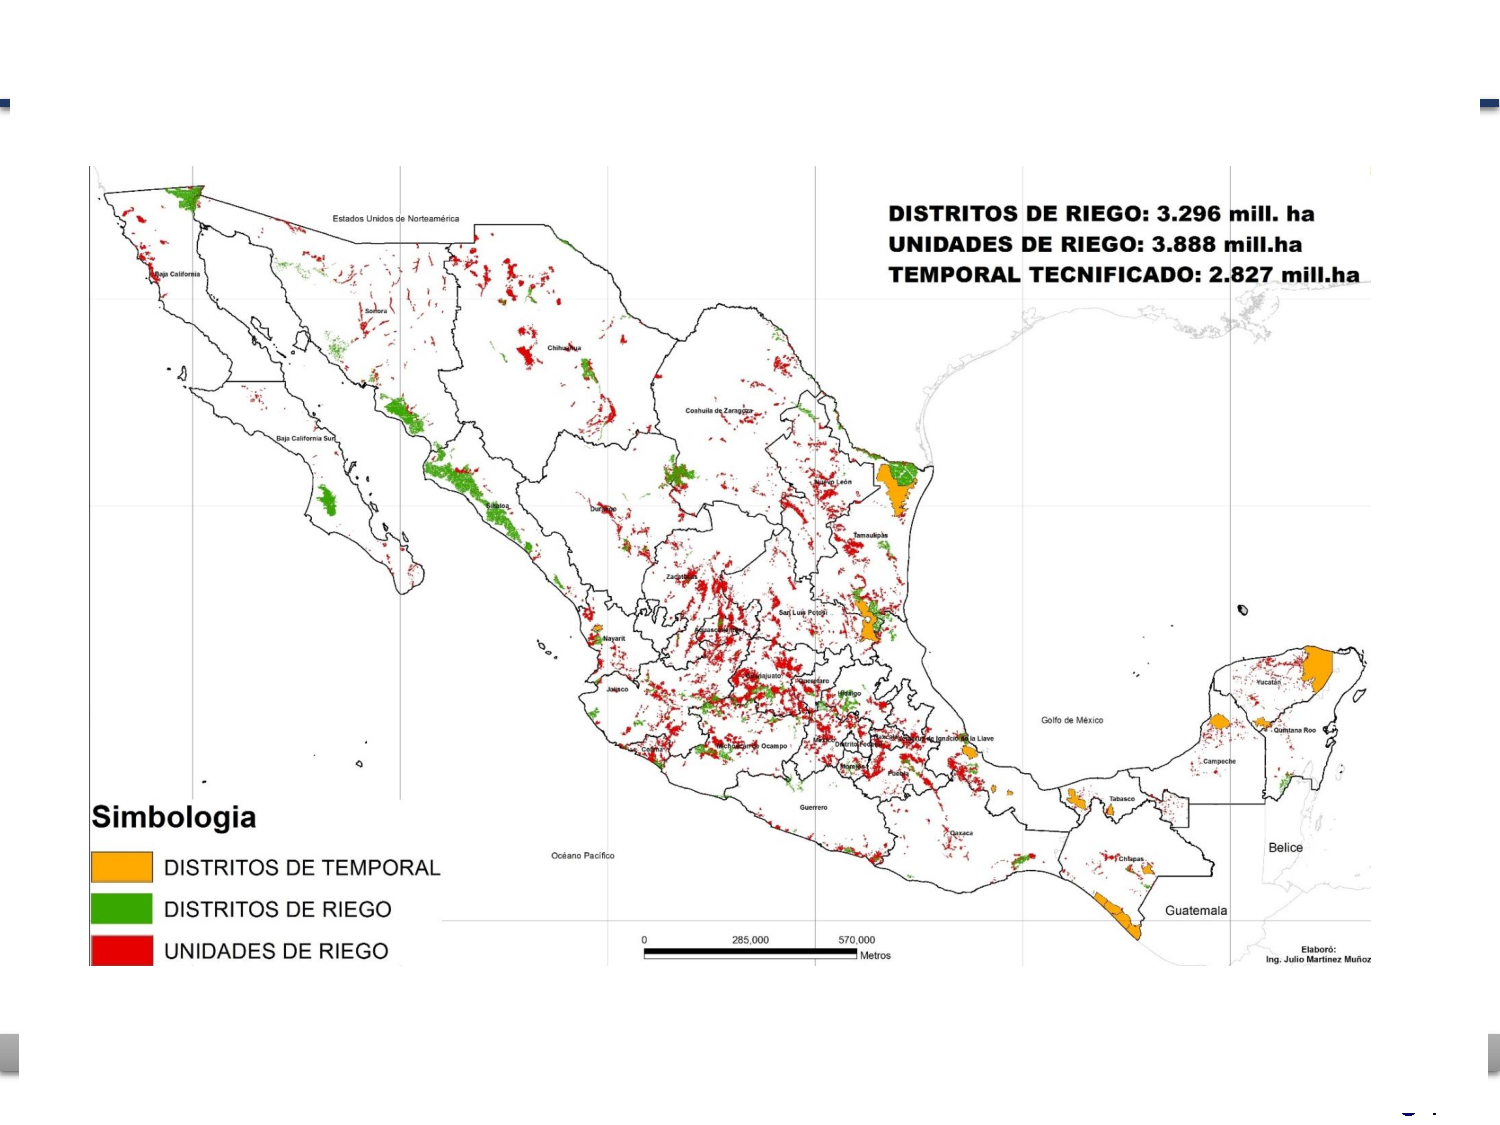
\includegraphics[width=0.5\textwidth]{ei2.pdf}
  \caption{Establecimiento de los Distritos de Temporales Tecnificado, Superficie con infraestructura Hidroagrícolas}
  \label{ie2}
\end{figure}

\begin{definition}[conservación Normal]
    Toda la infraestructura necesita un mantenimiento por año.
\end{definition}
\begin{definition}[Conservcaión diferida]
    Cuando la infraestructura ya está deteriorada y necesita una rehabilitación, pagado con los impuestos del pueblo de México
\end{definition}

\begin{table}[h!]
    \centering \begin{turn}{90}
    \begin{tabular}{@{}ccccccccc@{}}
    \toprule
    \multicolumn{2}{c}{\begin{tabular}[c]{@{}c@{}}Distrito de Temporal\\ Tecnificado\end{tabular}} &
      A.C.U. &
      Asociación Civil de Usuarios &
      Fecha de Constitución &
      \begin{tabular}[c]{@{}c@{}}Patronatos\\ (TOTAL)\end{tabular} &
      Patronatos &
      \begin{tabular}[c]{@{}c@{}}Usuarios\\ (TOTAL)\end{tabular} &
      Usuarios \\ \midrule
    011 &
      \begin{tabular}[c]{@{}c@{}}Margaritas-\\ Comitán\end{tabular} &
      1 &
      Meseta Comitéca A.C. &
      6/02/1997 &
      6 &
      6 &
      1402 &
      1402 \\
    012 &
      La Chontalpa &
      1 &
      El Plan Chontalpa Vive A.C. &
      23/01/2008 &
      22 &
      22 &
      8500 &
      8500 \\
    013 &
      \begin{tabular}[c]{@{}c@{}}Balancán-\\ Tecnosique\end{tabular} &
      1 &
      Nueva esperanza en el sur A.C. &
      12/12/2009 &
      29 &
      29 &
      2995 &
      2995 \\
    015 &
      \begin{tabular}[c]{@{}c@{}}Eszna-\\ Yohualtún\end{tabular} &
      1 &
      \begin{tabular}[c]{@{}c@{}}Valles Unidos de Eszná-\\ Yohualtún A.C.\end{tabular} &
      21/06/2004 &
      24 &
      24 &
      1706 &
      1706 \\
    016 &
      \begin{tabular}[c]{@{}c@{}}Sánes-\\ Huaesteca\end{tabular} &
      1 &
      Cuencas Sánes-Huastéca A.C. &
      22/04/2004 &
      5 &
      5 &
      2483 &
      2483 \\
    017 &
      Tapachula &
      1 &
      Usuarios del sur de Chiapas A.C. &
      14/02/1994 &
      10 &
      10 &
      8560 &
      8560 \\
    018 &
      Huixtla &
      1 &
      EL cigüeño A.C. &
      02/12/1993 &
      10 &
      10 &
      5858 &
      5858 \\
    020 &
      \begin{tabular}[c]{@{}c@{}}Margaritas-\\ Pijijiapan\end{tabular} &
      1 &
      La esperanza del año 2000 A.C. &
      03/09/1998 &
      4 &
      4 &
      1101 &
      1101 \\
    025 &
      Río Verde &
      1 &
      La esperanza del nuevo Milenio A.C. &
      3/12/1999 &
      20 &
      20 &
      1806 &
      1806 \\
    \multirow{2}{*}{026} &
      \multirow{2}{*}{Valle de Ucúm} &
      \multirow{2}{*}{2} &
      Cuna del mestizaje A.C. &
      26/01/2004 &
      \multirow{2}{*}{10} &
      5 &
      \multirow{2}{*}{1739} &
      973 \\
     &
       &
       &
      Central Flores, A.C. &
      26/01/2004 &
       &
      5 &
       &
      766 \\
    \multirow{2}{*}{027} &
      \multirow{2}{*}{Frailesca} &
      \multirow{2}{*}{2} &
      Los diez grandes de la frailesca A.C. &
      30/10/2003 &
      \multirow{2}{*}{8} &
      4 &
      \multirow{2}{*}{3850} &
      2204 \\
     &
       &
       &
      Cuenca baja santo domingo A.C. &
      29/10/2003 &
       &
      4 &
       &
      1646 \\
    035 &
      Los naranjos &
      1 &
      Costretib A.C. &
      17/03/2004 &
      15 &
      15 &
      6045 &
      60456 \\
     &
       &
       &
       &
       &
      413 &
      413 &
      110,825.0 &
      110,825.00 \\ \bottomrule
    \end{tabular} \end{turn}
    \caption{Organización de los distritos de temporal tecnificado}
    \label{tabeia1}
\end{table}


















